\section{Artificially expanding the size of the CA3 sub-field }
As the model is derived from the classical view of the hippocampus, the CA3 sub-field is represented by a TRBM.
The size of the CA3 sub-field is dependent on the environment being learned.
For example, the plus maze environment, \figureref{fig:plus_maze}, is made of 13 segments.
This gives us 13 nodes for position, and 52 nodes for the combination of position and direction headed.
In addition, the model allows for 4 nodes of sensory data, as well as the combination of sensor and direction which total 16.
Finally, we add in a bias node, which gives a base size of the CA3 of 86.


\begin{figure}
    \centering
    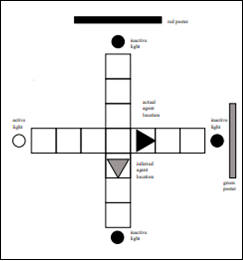
\includegraphics[width=0.5\textwidth]{figures/methods_size/plus_maze.png}
    \caption{The plus maze environment the model is learning, from \cite{foxandprescott2010A}}
    \label{fig:plus_maze}
\end{figure}

From how the CA3 sub-field is created, it provides two main options for increasing it's default size:
changing the environment the model learns and increasing the number of biases in the model.
Changing the environment would be impractical as multiple new environments that have different sizes would need to be created to fully explore how the time to learn changes as the CA3 sub-field increases in size.
On the other hand, increasing the number of biases in the model is trivial, and can be used to provide a comparison of how the time to learn is affected by multiple size changes to the CA3 sub-field.


% This makes the only options for increasing the size of the CA3 changing the environment the model learns, or increasing the number of bias nodes in the CA3 sub-field.
% Changing the environment would be impractical as a new environment of different size is needed to show how the model scales. 
% In addition, from how the CA3 is currently created, it is non-trivial to create a large environment for the model to learn.
%  \wording
% On the other hand, it can be considered trivial to add bias nodes to the creation of the CA3 sub-field.
% This allows for the model to be horizontally scaled quickly and easily, with the option to change the amount of extra nodes added.

We expect to see that the more nodes we add to the CA3, the time taken to train increases at a constant rate.
On the CPU version, we would expect to see a steep increase in time taken, whereas the GPU version would be a more gradual increase.


A problem that occurs when increasing the size of the CA3 sub-field is the increase in memory usage.
This is because Tensorflow converts from NumPy floating point arrays and Python floating point numbers to a 64 bit floating point tensor of the same size.
This is not suitable for GPU processing.
This is because GPU's have the best efficiency when working on 32 bit floating point numbers.
Whilst this change does reduce the overall precision of the model, for the purposes of this experiment, it can be considered to have a negligible effect on the results.

\subsection{Results from increasing the size of the CA3 sub-field}
% Plot this data as a graph? Might look better and would break the monotone document with some colour
As the number of neurons increases, the amount of calculations increases. 
Naturally this increases the amount of time the system needs to learn.
As can be seen from \tableref{tab:results_table_size}, increasing the size of the CA3 subfield also increases the time required to train the system.
\begin{table}[ht]
    \centering
        \begin{tabular}{|c|c|c|}
            \hline
            Number of Nodes in CA3 & Time Taken CPU (s) & Time Taken GPU (s) \\\hline
            86      & 83.3           & 335.6          \\ \hline
            1086    & 770.3          & 441.3          \\ \hline
            2086    & 2437.2         & 625.7          \\ \hline
            3086    & 4653.8         & 896.9          \\ \hline
            4086    & 7391.2         & 1231.5         \\ \hline
            5086    & 10337.4        & 1642.0         \\ \hline
            6086    & 14137.6        & 2154.4         \\ \hline
            7086    & 19531.4        & 2739.1         \\ \hline
            8086    & 24685.6        & 3423.7         \\ \hline
            9086    & 27058.8        & 4155.0         \\ \hline
        \end{tabular}
    \caption{
        Time taken to run the training process for different sizes of an artificially inflated CA3 using the model variations from test 0 and test 17.\footnotemark
    }
    \label{tab:results_table_size}
\end{table}



As we linearly increase the number of nodes from 3086, it requires approximately 3600 seconds (1 hour) more time.
In contrast, using the parallelised Tensorflow version, we only require approximately 420 seconds (7 minutes) more time for increased nodes.
This is a speed up of roughly 10 times for extra nodes.
These times were recorded on the implementations of Test ID 0 for the CPU version and Test ID 17 implementation for the GPU version.


\footnotetext{See \footref{foot:system} for system details.}